%% Discover Computing (Springer Nature) submission
%% Compiled with the Springer Nature sn-jnl.cls template, sn-mathphys reference style, numbered citations.
\documentclass[pdflatex,sn-mathphys,Numbered]{sn-jnl}

\usepackage{graphicx}
\usepackage{multirow}
\usepackage{amsmath,amssymb,amsfonts}
\usepackage{amsthm}
\usepackage{mathrsfs}
\usepackage[title]{appendix}
\usepackage{textcomp}
\usepackage{manyfoot}
\usepackage{xcolor}
\usepackage{geometry}
\usepackage{booktabs}
\usepackage{bm}
\usepackage{subfigure}
\usepackage{threeparttable}

\theoremstyle{thmstyleone}
\newtheorem{theorem}{Theorem}
\newtheorem{lemma}[theorem]{Lemma}
\newtheorem{corollary}[theorem]{Corollary}
\theoremstyle{thmstyletwo}
\newtheorem{remark}{Remark}
\theoremstyle{thmstylethree}
\newtheorem{definition}{Definition}

\raggedbottom

\begin{document}

\title[A Logarithmic Barrier Function-Based Newton's Model for Dynamic Quadratic Programming]{A Logarithmic Barrier Function-Based Newton's Model for Solving Dynamic Quadratic Programming Subject to Inequality Constraints}

\author*[1]{\fnm{Yuqun} \sur{Zhou}}\email{pkzyq1994@gmail.com}

\author[2]{\fnm{Jiufan} \sur{Wang}}\email{wang.18428@osu.edu}

\affil*[1]{\orgdiv{Department of Industrial and Systems Engineering}, \orgname{University of Wisconsin--Madison}, \orgaddress{\city{Madison}, \postcode{53706}, \state{WI}, \country{USA}}}

\affil[2]{\orgdiv{Department of Integrated Systems Engineering}, \orgname{The Ohio State University}, \orgaddress{\city{Columbus}, \postcode{43210}, \state{OH}, \country{USA}}}

\abstract{Time-critical computing systems -- from autonomous robots to intelligent transportation and traffic infrastructure -- increasingly rely on the real-time solution of quadratic programs whose objectives and inequality constraints evolve continuously with time. This paper introduces a logarithmic barrier function-based Newton (LBFN) computational model for solving such dynamic quadratic programs subject to inequality constraints (DQP-IC) without resorting to Karush--Kuhn--Tucker (KKT) reformulations or auxiliary dual variables. By embedding a parametric, adaptive logarithmic barrier directly into a continuous-time prediction-correction dynamical system, the LBFN model achieves (i)~convergence from arbitrary feasible or infeasible initializations, (ii)~global asymptotic stability, and (iii)~an exponentially decaying, tunable-rate tracking error, all supported by formal well-posedness and Lyapunov-based convergence proofs, together with an explicit, tunable-rate bound on the distance between the tracked trajectory and the true time-varying optimum. We additionally derive the per-iteration computational complexity of the proposed model and show that it matches that of a single dense Newton step, making it a practical computational primitive for embedded and edge-computing optimization pipelines. Extensive numerical comparisons against active-set, sequential quadratic programming, interior-point (SeDuMi), continuous gradient-descent, and Newton-flow solvers show that the LBFN model sustains lower tracking error and uninterrupted constraint satisfaction under fast parameter drift. A real-time robot navigation case study -- tracking a moving target while avoiding seven dynamic obstacles -- demonstrates the model's applicability to safety-critical autonomous computing systems.}

\keywords{Dynamic quadratic programming, inequality constraints, logarithmic barrier function, real-time computing, global convergence, robotic navigation}

\maketitle

\section{Introduction}\label{sec1}
Operating in highly dynamic environments, modern computing and control systems demand instantaneous adaptation of optimal decisions to rapidly changing conditions \cite{ldfy,acces23,trp2024}. This necessity for real-time adaptive programming is particularly critical in domains such as robotic autonomous navigation \cite{acceess4,trp2025,titis333} and intelligent traffic management systems \cite{acces345,titis2}. Effective operation of these systems hinges on the continuous computational resolution of programming problems with time-varying objectives and constraints. As applications increase in scale and complexity, the development of practical computational methodologies capable of accurately tracking optimal solutions under dynamic variations has become indispensable across computing infrastructures, from aerospace target-tracking and microgrid control pipelines \cite{tesagf, acceess3} to large-scale nonconvex optimization on networked computing systems \cite{TSTT12}.

Conventional strategies primarily address static programming problem formulations, where parameters remain fixed throughout the solution process \cite{tiify,siam1}. Techniques like gradient-flow dynamics utilize first-order descent principles for unconstrained minimization \cite{hwx2,aces355}, while Newton-type flows accelerate convergence by incorporating second-order curvature information \cite{trone3,newt1}. Constrained problems often employ active-set strategies \cite{act-se33,act-se} and sequential quadratic programming \cite{SQP3444, SQP34}. However, the above-mentioned approaches are proven effective for static programming problems; these approaches encounter limitations when deployed as computational modules inside dynamic systems with persistent parameter drift, because they lack an effective predictive mechanism to compensate for the solution drift \cite{S22, S44}.

A critical challenge arises because static solvers, when used as re-solved subroutines, lack temporal awareness. When applied to dynamic systems, treating each programming instance as an independent snapshot, they inevitably generate substantial tracking errors \cite{S4456,nn34, S4fw4}. For example, consider a robotic manipulator that moves between points while avoiding dynamically moving obstacles \cite{rbmm,rbm3Rm}. If its onboard path-planning computation uses a static optimizer without prediction, it would solve the problem only at the current instant based on the obstacle's current position. However, during the finite computation time, e.g., 50~ms, required to compute the optimal solution, both the robot and the obstacles have moved. The solution computed at $t_k$ is therefore optimized for a past state ($t_k$) and applied at a future state ($t_k$ + computation time), resulting in sub-optimality or, worse, constraint violation if the obstacle moved unexpectedly close during that interval \cite{rbmmr4,xy111}. Similarly, in automated lane-changing scenarios for autonomous vehicles, a static planner reacting only to the instantaneous relative positions of surrounding vehicles without anticipating their motion trends could fail to generate a safe and efficient trajectory when neighboring vehicles accelerate or decelerate unexpectedly during the planning computation \cite{tiv124}. These limitations highlight two critical computational gaps: a lack of inherent mechanism to compensate for the temporal drift of the optimal solution between the time computation starts and ends, and a reliance on strategies for handling inequality constraints via KKT-based reformulations that are computationally expensive to recompute at every control cycle or that introduce additional auxiliary variables, complicating real-time deployment \cite{lfyy12,lj11}.

Beyond robotics and transportation, this same drift-and-constraint challenge underlies a broad class of continuously reconfigured decision problems in modern computing systems, including receding-horizon and model-predictive controllers that must re-solve quadratic subproblems every sampling interval, and edge- or embedded-computing pipelines that allocate limited resources under time-varying, hard operational bounds. In all such settings, a computational optimization primitive that both tolerates aggressive parameter drift and avoids the bookkeeping overhead of auxiliary dual variables is of direct practical value, since it lowers the per-iteration computational burden that ultimately governs achievable sampling rates on resource-constrained computing hardware -- directly relevant to the design of resilient computing infrastructure.

To address these limitations, this paper proposes a logarithmic barrier function-based Newton's (LBFN) model for dynamic inequality-constrained quadratic programming. Departing from the conventional paradigm of converting inequalities into equality systems via KKT conditions, which requires the introduction of dual variables, the LBFN model employs parametric adaptive log-barrier functions to directly incorporate dynamic inequality constraints. This formulation fundamentally avoids the need for auxiliary variables. The proposed model integrates a prediction mechanism that estimates the future drift of the optimal solution using time derivatives of the problem parameters, along with a Newton-based correction dynamics that drives the solution toward the optimum of the barrier-augmented objective while ensuring continuous constraint satisfaction throughout the evolution. The main contributions of this work are summarized as follows:

\begin{itemize}
\item A novel LBFN computational model is constructed for real-time solving of dynamic quadratic programming subject to inequality constraints (DQP-IC), which employs parametric adaptive log-barrier functions instead of KKT-based constraint handling.

\item The LBFN model exhibits initialization insensitivity, enabling convergence to the optimal trajectory from arbitrary initial points (feasible or infeasible), while maintaining exponentially decaying tracking errors with a tunable convergence rate. We formally establish the well-posedness of the model and derive its per-iteration computational complexity, which is comparable to that of a single Newton step on a static quadratic program.

\item Theoretical analysis, numerical simulations against five established solvers, and a real-time robotic navigation application are presented to validate the effectiveness and computational advantages of the proposed approach, together with a discussion of the model's limitations and directions for future work.
\end{itemize}

\textbf{Notation:} For any dynamic vector $\bm{v}(t) \in \mathbb{R}^{n}$, the Euclidean norm is expressed as $\|\bm{v}(t)\|_{2}$. Consider a function $\hbar(\bm{v}(t), t)$. The optimal value of this function is denoted by $\hbar(\bm{v}^{*}(t),t)$, where $\bm{v}^{*}(t)$ signifies the optimal trajectory of the decision variable $\bm{v}(t)$. The gradient of $\hbar$ with respect to $\bm{v}(t)$ is represented by $\nabla_{\bm{v}}\hbar(\bm{v}(t), t)$, and its partial derivative with respect to time $t$ is given by $\partial_{t}\hbar(\bm{v}(t), t)$. The Hessian matrix of $\hbar$ with respect to $\bm{v}(t)$ is denoted by $\nabla_{\bm{vv}}\hbar(\bm{v}(t), t)$. Furthermore, the partial derivative of the gradient $\nabla_{\bm{v}}\hbar(\bm{v}(t), t)$ with respect to $t$ is written as $\nabla_{\bm{vt}}\hbar(\bm{v}(t), t)$. The $i$-th component of the vector $\bm{v}(t)$ is indicated by $\bm{v}_{i}(t)$, and $\mathbb{S}^n_{++}$ denotes the cone of $n\times n$ symmetric positive-definite matrices.

\section{Preliminary and Scheme Formulation}\label{sec2}
In this part, the dynamic quadratic programming problem subject to inequality constraints and the LBFN model preliminaries are provided in detail.

\subsection{Construction of the DQP-IC Problem}\label{subsec21}
Consider a DQP-IC problem formulated as:
\begin{equation}
\begin{aligned}
& \underset{\bm{v}(t) \in \mathbb{R}^n}{\text{minimize}} & & \hbar(\bm{v}(t), t) = \frac{1}{2} \bm{v}^\top(t) \mathcal{M}(t) \bm{v}(t) + \bm{g}^\top(t)\bm{v}(t) \\
& \text{subject to} & & \mathcal{N}(t) \bm{v}(t) \leq \bm{d}(t)
\end{aligned}
\label{eq:problem}
\end{equation}
where $\bm{v}(t) \in \mathbb{R}^n$ is a decision variable. $t \geq 0$ denotes continuous time. $\mathcal{M}(t) \in \mathbb{S}^n_{++}$ is a symmetric positive-definite matrix with $\mathcal{M}(t) \succeq m_f \mathcal{I}_n$ for some $m_f > 0$ (uniform strong convexity). $\bm{g}(t) \in \mathbb{R}^n$ is a dynamic linear coefficient vector. $\mathcal{N}(t) \in \mathbb{R}^{p \times n}$ and $\bm{d}(t) \in \mathbb{R}^p$ define $p$ linear inequality constraints, with $\mathcal{A}_i(t)$ denoting the $i$-th row of $\mathcal{N}(t)$ and $d_i(t)$ the $i$-th entry of $\bm{d}(t)$. All problem data $\mathcal{M}(t)$, $\bm{g}(t)$, $\mathcal{N}(t)$, $\bm{d}(t)$ and their first time derivatives are assumed continuous and available in closed form. The feasible set $\mathcal{F}(t) = \{\bm{v}(t) \in \mathbb{R}^n : \mathcal{N}(t) \bm{v}(t) \leq \bm{d}(t)\}$ satisfies Slater's condition for all $t \geq 0$.

To handle constraints, we introduce a dynamic barrier parameter $w(t) > 0$ with $w(t) = w(0)e^{\gamma_w t}$, $\gamma_w>0$, so that $\lim_{t \to \infty} w(t) = \infty$, and a dynamic slack variable $r(t) > 0$ with $r(t) = r(0)e^{-\gamma_r t}$, $\gamma_r > 0$, ensuring $r(t) \to 0$ asymptotically.
The modified objective $\Upsilon(\bm{v}(t), w(t), r(t), t)$ is defined as:
\begin{equation}
\begin{aligned}
\Upsilon(\bm{v}(t), w(t), r(t), t) = \hbar(\bm{v}(t), t) - \frac{1}{w(t)} \sum_{i=1}^p \log \bigg( r(t) - \big( \mathcal{A}_i(t) \bm{v}(t) - d_i(t) \big) \bigg)
\end{aligned}
\label{eq:psi}
\end{equation}
The domain $\widehat{\mathcal{D}}(t) = \{ \bm{v}(t) \in \mathbb{R}^n : \mathcal{A}_i(t) \bm{v}(t) - d_i(t) < r(t),\ i=1,\dots,p \}$ is non-empty when $r(0) > \max_i (\mathcal{A}_i(0) \bm{v}(0) - d_i(0))$.

\subsection{General Framework of the LBFN Model}\label{subsec22}
Then, an implicit evolution dynamics is constructed as:
\begin{equation}
\dot{\bm{v}}(t) = -\nabla_{\bm{v}\bm{v}}^{-1} \Upsilon \left[ \alpha \nabla_{\bm{v}} \Upsilon + \nabla_{\bm{v} r} \Upsilon \dot{r} + \nabla_{\bm{v} w} \Upsilon \dot{w} + \nabla_{\bm{v} t} \Upsilon \right]
\label{eq:dynamics}
\end{equation}
where $\alpha > 0$ is a convergence rate parameter. $\nabla_{\bm{v} \bm{v}}\Upsilon$ is the Hessian of $\Upsilon$ w.r.t. $\bm{v}(t)$. $\nabla_{\bm{v}}\Upsilon$, $\nabla_{\bm{v} r}\Upsilon$, $\nabla_{\bm{v} w}\Upsilon$, and $\nabla_{\bm{v} t}\Upsilon$ are partial derivatives.

Define $\delta_i(\bm{v}(t),t)=r(t)-(\mathcal{A}_i(t)\bm{v}(t)-d_i(t))$, and the following definitions are given:
\begin{equation}
\nabla_{\bm{v}} \Upsilon = \mathcal{M}(t) \bm{v}(t) + \bm{g}(t) + \frac{1}{w(t)} \sum_{i=1}^{p} \frac{\mathcal{A}_i(t)^\top}{\delta_i(\bm{v}(t), t)}
\label{eq:grad_psi_u}
\end{equation}

\begin{equation}
\nabla_{\bm{v}\bm{v}} \Upsilon = \mathcal{M}(t) + \frac{1}{w(t)} \sum_{i=1}^{p} \frac{\mathcal{A}_i(t)^\top \mathcal{A}_i(t)}{\delta_i^2(\bm{v}(t), t)}
\label{eq:hessian_psi_uu}
\end{equation}

\begin{equation}
\nabla_{\bm{v} r} \Upsilon = \frac{1}{w(t)} \sum_{i=1}^{p} \frac{\mathcal{A}_i(t)^\top}{\delta_i^2(\bm{v}(t), t)}
\label{eq:grad_psi_ur}
\end{equation}

\begin{equation}
\nabla_{\bm{v} w} \Upsilon = -\frac{1}{w^2(t)} \sum_{i=1}^{p} \frac{\mathcal{A}_i(t)^\top}{\delta_i(\bm{v}(t), t)}
\label{eq:grad_psi_uw}
\end{equation}

\begin{equation}
\begin{aligned}
\nabla_{\bm{v} t} \Upsilon = \dot{\mathcal{M}}(t) \bm{v}(t) + \dot{\bm{g}}(t) + \frac{1}{w(t)} \sum_{i=1}^{p} \frac{\dot{\mathcal{A}}_i(t)^\top}{\delta_i(\bm{v}(t), t)}
+ \frac{1}{w(t)} \sum_{i=1}^{p} \frac{\mathcal{A}_i(t)^\top \left( \dot{\mathcal{A}}_i(t) \bm{v}(t) - \dot{d}_i(t) \right)}{\delta_i^2(\bm{v}(t), t)}
\end{aligned}
\label{eq:grad_psi_ut}
\end{equation}

Substituting into \eqref{eq:dynamics}, it is eventually obtained the following LBFN model:
\begin{equation}
\begin{aligned}
\dot{\bm{v}}(t)=  &-\bigg( \mathcal{M}(t) + \frac{1}{w(t)} \sum_{i=1}^{p} \frac{\mathcal{A}_i(t)^\top \mathcal{A}_i(t)}{\delta_i^2(\bm{v}(t), t)} \bigg)^{-1} \bigg( \alpha \bigg( \mathcal{M}(t) \bm{v}(t)+ \bm{g}(t)+ \frac{1}{w(t)} \sum_{i=1}^{p} \frac{\mathcal{A}_i(t)^\top}{\delta_i(\bm{v}(t), t)} \bigg) \\
&+ \left( \frac{1}{w(t)} \sum_{i=1}^{p} \frac{\mathcal{A}_i(t)^\top}{\delta_i^2(\bm{v}(t), t)} \right) \dot{r}(t)+ \left( -\frac{1}{w^2(t)} \sum_{i=1}^{p} \frac{\mathcal{A}_i(t)^\top}{\delta_i(\bm{v}(t), t)} \right) \dot{w}(t) + \nabla_{\bm{v} t} \Upsilon \bigg)
\end{aligned}
\label{eq:full_dynamics}
\end{equation}
where $\dot{r}(t)=-\gamma_r r(t)$ and $\dot{w}(t)=\gamma_w w(t)$ follow directly by differentiating $r(t)=r(0)e^{-\gamma_r t}$ and $w(t)=w(0)e^{\gamma_w t}$, respectively.

While \eqref{eq:problem} restricts $\hbar$ to be quadratic so that \eqref{eq:full_dynamics} admits the closed form above and the theoretical analysis of Section~\ref{sec3} applies directly, the underlying implicit dynamics \eqref{eq:dynamics} are not intrinsically limited to quadratic objectives: for any $\hbar(\bm{v}(t),t)$ that is twice continuously differentiable and $m_f$-strongly convex in $\bm{v}(t)$ for every $t$, substituting the general $\nabla_{\bm{v}}\hbar$, $\nabla_{\bm{vv}}\hbar$, and $\nabla_{\bm{vt}}\hbar$ for $\mathcal{M}(t)\bm{v}(t)+\bm{g}(t)$, $\mathcal{M}(t)$, and $\dot{\mathcal{M}}(t)\bm{v}(t)+\dot{\bm{g}}(t)$ in \eqref{eq:grad_psi_u}--\eqref{eq:grad_psi_ut} yields the same prediction-correction structure, and Lemma~\ref{lem:wellposed}, Theorem~\ref{thm:main}, and Corollary~\ref{cor:tracking} continue to hold verbatim with $\hbar$ in place of the quadratic form, provided $\hbar(\cdot,t)$ remains $m_f$-strongly convex for every $t$. Section~\ref{subsec42} uses this more general instantiation for a non-quadratic potential-field objective that is only locally, not globally, strongly convex (Section~\ref{sec5}); that case study therefore demonstrates the LBFN mechanism empirically beyond the setting formally covered by Theorem~\ref{thm:main}, as is standard practice for this class of computational optimization primitives applied to real-world potential-field navigation tasks.

\section{Theoretical Analysis}\label{sec3}
This part provides the theoretical analysis for the LBFN model \eqref{eq:full_dynamics}, including its well-posedness, global convergence, and computational complexity -- the last of which is of direct interest for real-time computing deployment.

\begin{lemma}[Well-posedness]\label{lem:wellposed}
For every $t\geq0$ and every $\bm{v}(t)\in\widehat{\mathcal{D}}(t)$, the Hessian $\nabla_{\bm{vv}}\Upsilon(\bm{v}(t),w(t),r(t),t)$ in \eqref{eq:hessian_psi_uu} is symmetric positive definite, and the right-hand side of \eqref{eq:full_dynamics} is locally Lipschitz continuous in $\bm{v}(t)$ on $\widehat{\mathcal{D}}(t)$. Consequently, for any $\bm{v}(0)\in\widehat{\mathcal{D}}(0)$ the LBFN model \eqref{eq:full_dynamics} admits a unique solution trajectory $\bm{v}(t)$ that remains in $\widehat{\mathcal{D}}(t)$ for all $t\geq0$.
\end{lemma}
\begin{proof}
By assumption $\mathcal{M}(t)\succeq m_f\mathcal{I}_n\succ0$. For $\bm{v}(t)\in\widehat{\mathcal{D}}(t)$, $\delta_i(\bm{v}(t),t)>0$ for every $i$, so each rank-one term $\mathcal{A}_i(t)^\top\mathcal{A}_i(t)/\delta_i^2(\bm{v}(t),t)$ in \eqref{eq:hessian_psi_uu} is symmetric positive semidefinite; a sum of a positive-definite matrix and positive-semidefinite matrices is positive definite, so $\nabla_{\bm{vv}}\Upsilon\succeq m_f\mathcal{I}_n\succ0$ and is therefore invertible with $\|\nabla_{\bm{vv}}^{-1}\Upsilon\|_2\leq1/m_f$. Because $\Upsilon$ is twice continuously differentiable on $\widehat{\mathcal{D}}(t)$ (all barrier terms are smooth away from the boundary $\delta_i=0$), the right-hand side of \eqref{eq:full_dynamics}, being a composition of continuously differentiable maps with the uniformly bounded inverse $\nabla_{\bm{vv}}^{-1}\Upsilon$, is locally Lipschitz in $\bm{v}(t)$ on any compact subset of $\widehat{\mathcal{D}}(t)$. Existence and uniqueness of a local solution then follow from the Picard--Lindel\"of theorem on any compact subset of $\widehat{\mathcal{D}}(t)$; Corollary~\ref{cor:tracking} below shows this local solution never approaches the boundary $\delta_i\to0^+$ in finite time and hence extends to all $t\geq0$.
\end{proof}

\begin{theorem}[Global exponential convergence]\label{thm:main}
Consider the LBFN model \eqref{eq:full_dynamics} for the DQP-IC problem \eqref{eq:problem}. Define the Lyapunov function candidate:
\begin{equation}
V(t) = \frac{1}{2} \| \nabla_{\bm{v}} \Upsilon(\bm{v}(t), w(t), r(t), t) \|_2^2
\label{eq:lyap}
\end{equation}
For any initial condition $\bm{v}(0)\in\widehat{\mathcal{D}}(0)$, $V(t)$ satisfies $\dot{V}(t) = -2\alpha V(t)$ for as long as the solution exists, and consequently $\lim_{t \to \infty} \| \nabla_{\bm{v}} \Upsilon(\bm{v}(t), w(t), r(t), t) \|_2 = 0$, i.e., the tracking error vanishes uniformly for every initial condition, regardless of how far $\bm{v}(0)$ starts from optimality.
\end{theorem}

\begin{figure*}[thbp]\centering
\subfigure[]{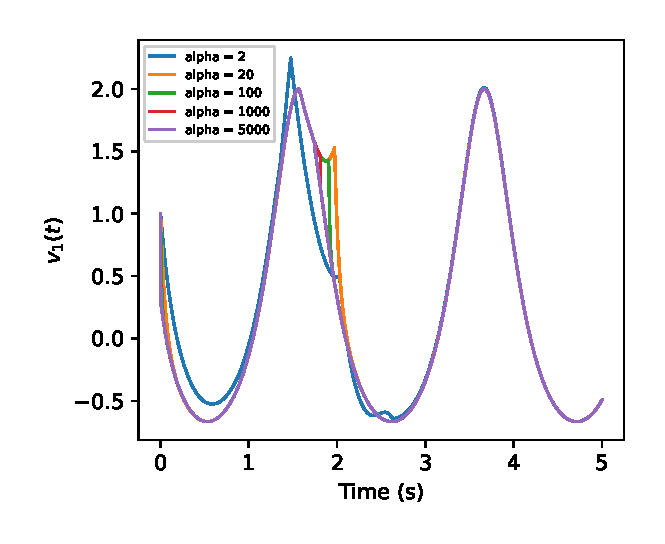
\includegraphics[width=58mm,height=46mm]{coeff_x1.eps}}
\subfigure[]{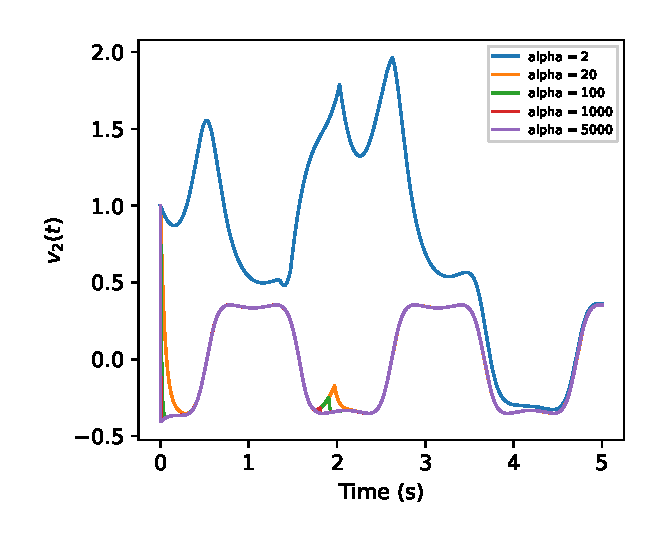
\includegraphics[width=58mm,height=46mm]{coeff_x2.eps}}
\subfigure[]{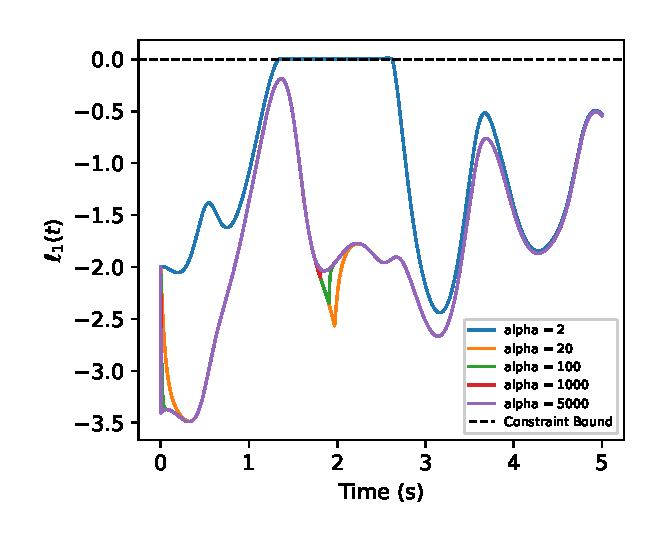
\includegraphics[width=58mm,height=46mm]{coeff_g1.eps}}
\subfigure[]{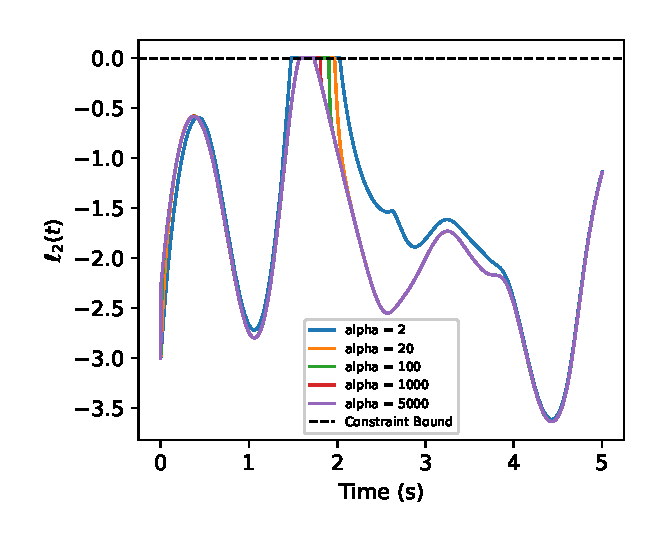
\includegraphics[width=58mm,height=46mm]{coeff_g2.eps}}
\subfigure[]{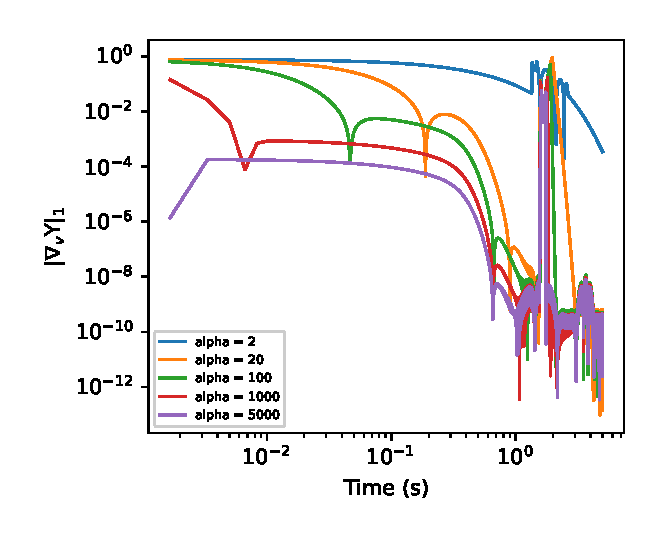
\includegraphics[width=58mm,height=46mm]{coeff_err1.eps}}
\subfigure[]{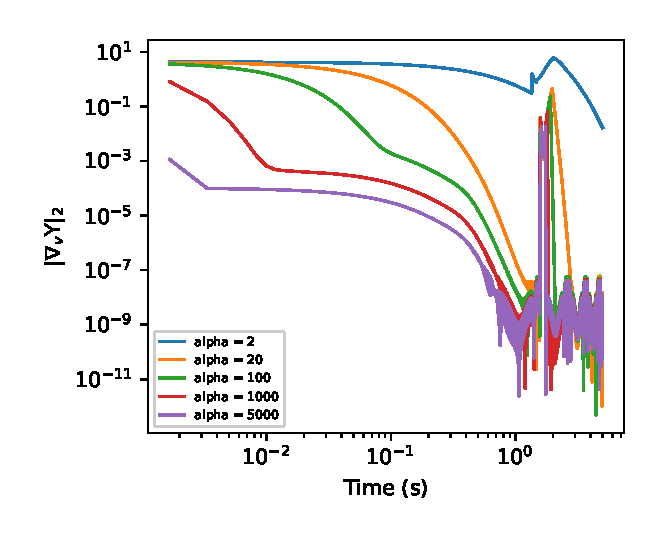
\includegraphics[width=58mm,height=46mm]{coeff_err2.eps}}
\caption{Simulative outcomes of the presented LBFN model \eqref{eq:full_dynamics} for the DQP-IC problem \eqref{eq:problem234}, with convergence parameter $\alpha$ varying from $2$ to $5000$, $\gamma_w=10$ and $\gamma_r=5$. (a) Convergence of $v_1(t)$. (b) Convergence of $v_2(t)$. (c) Constraint behavior of $g_1(t)= \sin(2t)v_1(t) + v_2(t)- (2 + \cos(2t))$. (d) Constraint behavior of $g_2(t)=-\cos(2t)v_1(t) + (2t/10)v_2(t)-(2 - \sin(4t))$. (e) First entry of the absolute gradient error. (f) Second entry of the absolute gradient error.}
\label{F333}
\end{figure*}

\begin{proof}
By Lemma~\ref{lem:wellposed}, $\nabla_{\bm{vv}}\Upsilon$ is invertible along the trajectory, so \eqref{eq:dynamics} is well defined. The time derivative of $V(t)$ is computed as:
\begin{equation}
\dot{V}(t) = \nabla_{\bm{v}} \Upsilon^\top \left( \frac{d}{dt} \nabla_{\bm{v}} \Upsilon \right)
\label{eq:vdot}
\end{equation}
The total derivative $\frac{d}{dt}\nabla_u\Upsilon$ expands to:
\begin{equation}
\frac{d}{dt} \nabla_{\bm{v}} \Upsilon = \nabla_{\bm{v}\bm{v}} \Upsilon  \dot{\bm{v}} + \nabla_{\bm{v} r} \Upsilon \dot{r} + \nabla_{\bm{v} w} \Upsilon  \dot{w} + \nabla_{\bm{v} t} \Upsilon
\label{eq:total_grad}
\end{equation}
Substitute the dynamics \eqref{eq:dynamics} into \eqref{eq:total_grad}:
\begin{equation}
\begin{aligned}
\frac{d}{dt} \nabla_{\bm{v}} \Upsilon = \nabla_{\bm{v}\bm{v}} \Upsilon \bigg( -\nabla_{\bm{v}\bm{v}}^{-1} \Upsilon \big( \alpha \nabla_{\bm{v}} \Upsilon + \nabla_{\bm{v} r} \Upsilon \dot{r}+\nabla_{\bm{v} w} \Upsilon \dot{w}  + \nabla_{\bm{v} t} \Upsilon \big) \bigg) + \nabla_{\bm{v} r} \Upsilon \dot{r} + \nabla_{\bm{v} w} \Upsilon \dot{w} + \nabla_{\bm{v} t} \Upsilon
\end{aligned}
\end{equation}
Simplify the expression:
\begin{equation}
\frac{d}{dt} \nabla_{\bm{v}} \Upsilon = -\alpha \nabla_{\bm{v}} \Upsilon - \nabla_{\bm{v} t} \Upsilon + \nabla_{\bm{v} t} \Upsilon = -\alpha \nabla_{\bm{v}} \Upsilon
\label{eq:simplified_total}
\end{equation}
The cancellation occurs because the prediction terms $(\nabla_{\bm{v}r}\Upsilon\dot{r}+\nabla_{\bm{v}w}\Upsilon\dot{w}+\nabla_{\bm{v}t}\Upsilon)$ are exactly compensated by the additional derivatives in the total derivative. This is a key feature of the prediction-correction structure. Substitute \eqref{eq:simplified_total} into \eqref{eq:vdot}:
\begin{equation}
\dot{V}(t) = \nabla_{\bm{v}} \Upsilon^\top \left( -\alpha \nabla_{\bm{v}} \Upsilon \right) = -2\alpha V(t)
\label{eq:vdot_ideal}
\end{equation}
Solving this ODE gives \cite{book12}:
\begin{equation}
V(t) = V(0) e^{-2\alpha t}
\label{eq:exp_decay}
\end{equation}
which implies $\lim_{t\to\infty}V(t)=0$, proving the theorem.
\end{proof}

\begin{corollary}[Tracking error relative to the true optimal trajectory]\label{cor:tracking}
Let $\bm{v}^*_\Upsilon(t):=\arg\min_{\bm{v}}\Upsilon(\bm{v},w(t),r(t),t)$ denote the instantaneous minimizer of the barrier-augmented objective and $\bm{v}^*(t)$ the true minimizer of \eqref{eq:problem}. Then
\begin{equation}
\|\bm{v}(t)-\bm{v}^*(t)\|_2 \;\leq\; \frac{\sqrt{2V(0)}}{m_f}\,e^{-\alpha t} \;+\; \sqrt{\frac{2p}{m_f\,w(0)}}\,e^{-\gamma_w t/2},
\label{eq:tracking_bound}
\end{equation}
so $\bm{v}(t)$ converges to the true time-varying optimal trajectory at rate $\min(\alpha,\gamma_w/2)$ -- both independently tunable -- and in particular $\bm{v}(t)$ remains within a bounded, shrinking distance of $\bm{v}^*(t)$ for all $t\geq0$ (hence never approaches $\partial\widehat{\mathcal{D}}(t)$ in finite time, completing the proof of Lemma~\ref{lem:wellposed}).
\end{corollary}
\begin{proof}
By Lemma~\ref{lem:wellposed}, $\Upsilon(\cdot,w(t),r(t),t)$ is $m_f$-strongly convex in $\bm{v}$ for every $t$, so the standard strong-convexity gradient inequality gives $\|\bm{v}(t)-\bm{v}^*_\Upsilon(t)\|_2\leq\frac{1}{m_f}\|\nabla_{\bm{v}}\Upsilon(\bm{v}(t),t)\|_2=\frac{\sqrt{2V(t)}}{m_f}=\frac{\sqrt{2V(0)}}{m_f}e^{-\alpha t}$ by Theorem~\ref{thm:main}. Separately, $\bm{v}^*_\Upsilon(t)$ is feasible for \eqref{eq:problem}, and the classical log-barrier suboptimality bound \cite{book12} gives $\hbar(\bm{v}^*_\Upsilon(t),t)-\hbar(\bm{v}^*(t),t)\leq p/w(t)$; since $\hbar(\cdot,t)$ is itself $m_f$-strongly convex ($\mathcal{M}(t)\succeq m_f\mathcal{I}_n$) and $\bm{v}^*(t)$ minimizes $\hbar(\cdot,t)$ over the feasible set, $\frac{m_f}{2}\|\bm{v}^*_\Upsilon(t)-\bm{v}^*(t)\|_2^2\leq\hbar(\bm{v}^*_\Upsilon(t),t)-\hbar(\bm{v}^*(t),t)\leq p/w(t)$, i.e. $\|\bm{v}^*_\Upsilon(t)-\bm{v}^*(t)\|_2\leq\sqrt{2p/(m_f w(t))}=\sqrt{2p/(m_f w(0))}\,e^{-\gamma_w t/2}$. The triangle inequality $\|\bm{v}(t)-\bm{v}^*(t)\|_2\leq\|\bm{v}(t)-\bm{v}^*_\Upsilon(t)\|_2+\|\bm{v}^*_\Upsilon(t)-\bm{v}^*(t)\|_2$ then yields \eqref{eq:tracking_bound}. Since the right-hand side is finite and continuous for all $t\geq0$, $\bm{v}(t)$ remains a bounded distance from the strictly feasible $\bm{v}^*_\Upsilon(t)$ on every compact time interval, so the local solution of Lemma~\ref{lem:wellposed} cannot cease to exist at any finite $t$.
\end{proof}

\subsection{Computational Complexity Analysis}\label{subsec31}
We next characterize the per-instant computational cost of evaluating \eqref{eq:full_dynamics}, which governs its suitability for real-time computing deployment. Let $n$ denote the decision-variable dimension and $p$ the number of inequality constraints. Forming the Hessian $\nabla_{\bm{vv}}\Upsilon$ in \eqref{eq:hessian_psi_uu} requires summing $p$ rank-one outer products $\mathcal{A}_i(t)^\top\mathcal{A}_i(t)$, each costing $O(n^2)$ operations, for a total of $O(pn^2)$; forming the gradient terms \eqref{eq:grad_psi_u}--\eqref{eq:grad_psi_ut} costs $O(pn)$. Since $\nabla_{\bm{vv}}\Upsilon$ is symmetric positive definite by Lemma~\ref{lem:wellposed}, the linear solve implicit in \eqref{eq:dynamics} can be carried out by Cholesky factorization at a cost of $O(n^3)$ rather than by an explicit matrix inversion, and the factorization can be reused across the right-hand-side terms sharing the same Hessian at a given instant \cite{book12}. The overall per-instant complexity of the LBFN update is therefore
\begin{equation}
O(n^3 + pn^2),
\label{eq:complexity}
\end{equation}
which is dominated by the $O(n^3)$ factorization step whenever $p=O(n)$, matching the cost of a single Newton step for a static quadratic program of the same size -- a favorable property for embedding the LBFN update inside a fixed-rate real-time computing loop. This compares favorably with KKT-based dynamic solvers, whose per-instant cost includes forming and factorizing an augmented system of dimension $n+p$ (or $n+2p$ when slack variables are introduced), and with active-set methods, whose worst-case combinatorial search over constraint activity has cost that grows with the number of candidate active sets rather than polynomially in $n$ and $p$. When $n$ is large, the $O(n^3)$ factorization cost can be further reduced using rank-one Hessian updates via the Sherman--Morrison--Woodbury identity or warm-started factorizations that exploit the continuity of $\nabla_{\bm{vv}}\Upsilon(t)$ across nearby time instants; we return to this point in Section~\ref{sec5}.

\begin{figure*}[thbp]\centering
\subfigure[]{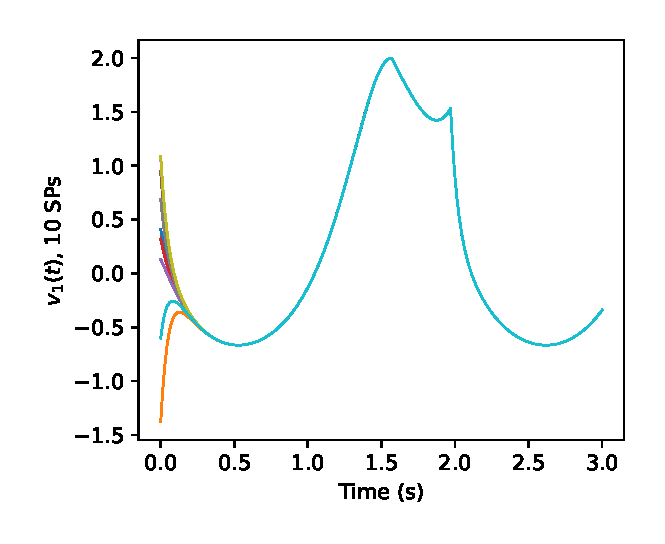
\includegraphics[width=58mm,height=46mm]{init_x1.eps}}
\subfigure[]{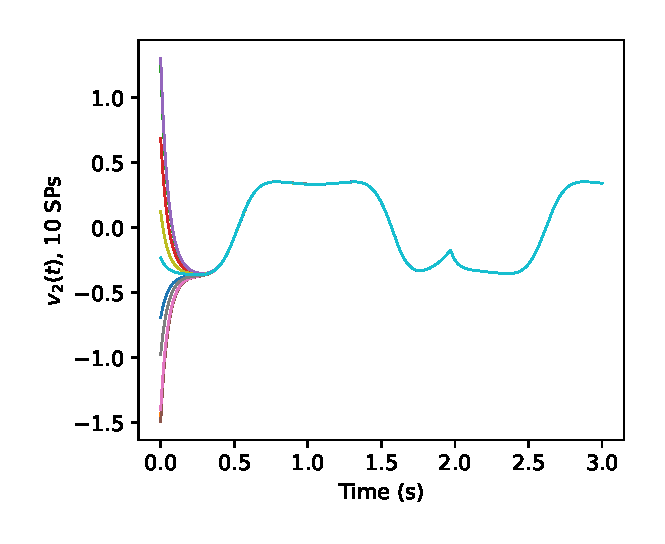
\includegraphics[width=58mm,height=46mm]{init_x2.eps}}
\subfigure[]{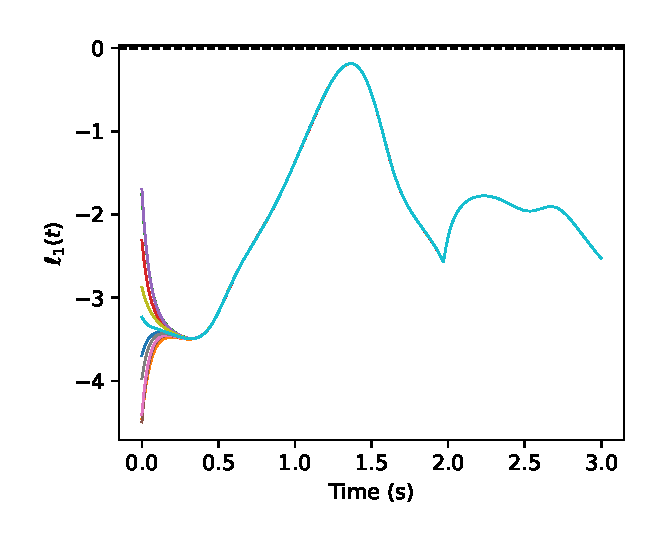
\includegraphics[width=58mm,height=46mm]{init_g1.eps}}
\subfigure[]{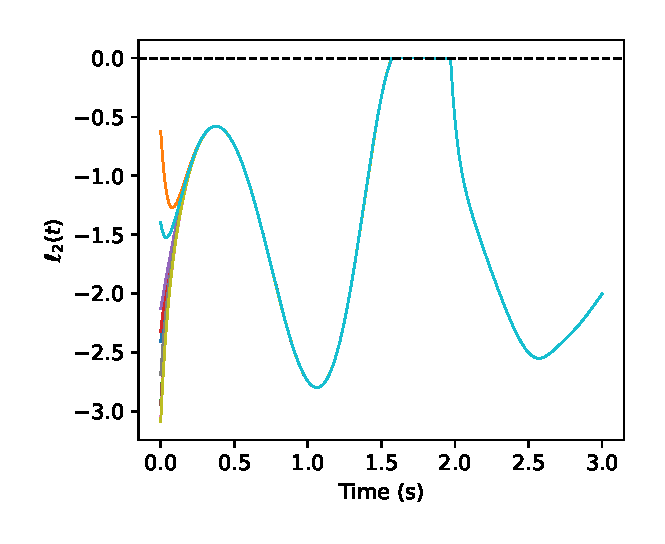
\includegraphics[width=58mm,height=46mm]{init_g2.eps}}
\subfigure[]{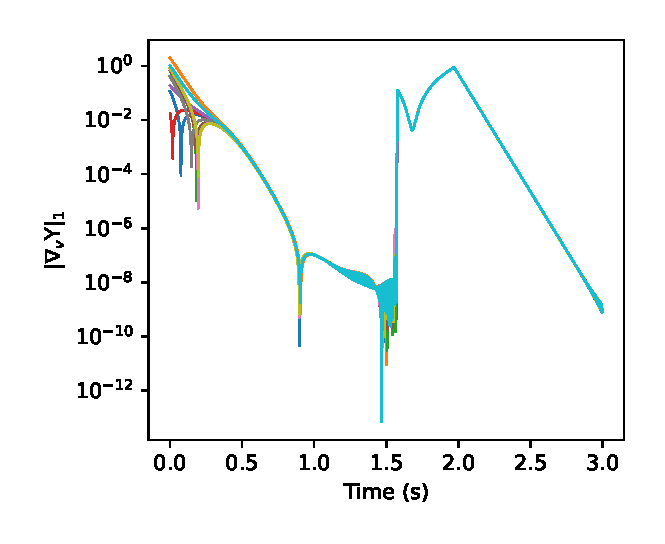
\includegraphics[width=58mm,height=46mm]{init_err1.eps}}
\subfigure[]{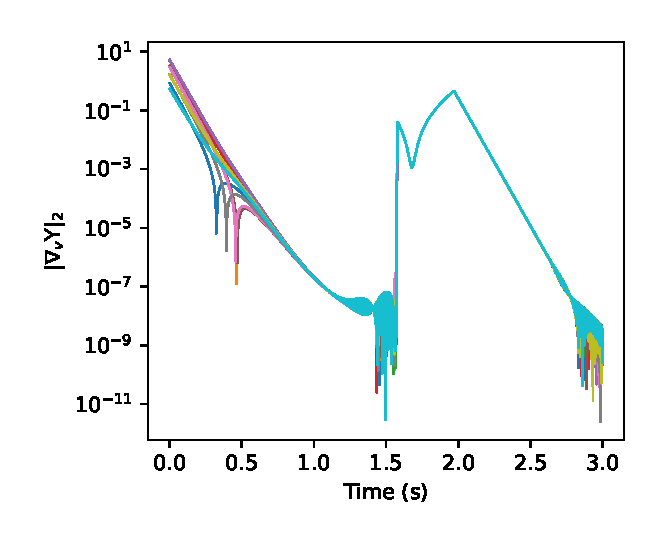
\includegraphics[width=58mm,height=46mm]{init_err2.eps}}
\caption{Simulative outcomes of the presented LBFN model \eqref{eq:full_dynamics} for the DQP-IC problem \eqref{eq:problem234}, under 10 different starting points (SP9 with $\bm{v}_i(0)\in[-1.5,1.5]$ sampled at random, plus one deliberately infeasible starting point $\bm{v}(0)=(-3,4)$), convergence parameter $\alpha=20$, $\gamma_w=10$ and $\gamma_r=5$. (a) Convergence of $v_1(t)$. (b) Convergence of $v_2(t)$. (c) Constraint behavior of $g_1(t)$. (d) Constraint behavior of $g_2(t)$. (e) First entry of the absolute gradient error. (f) Second entry of the absolute gradient error.}
\label{Fg3233}
\end{figure*}

\begin{figure*}[thbp]\centering
\subfigure[]{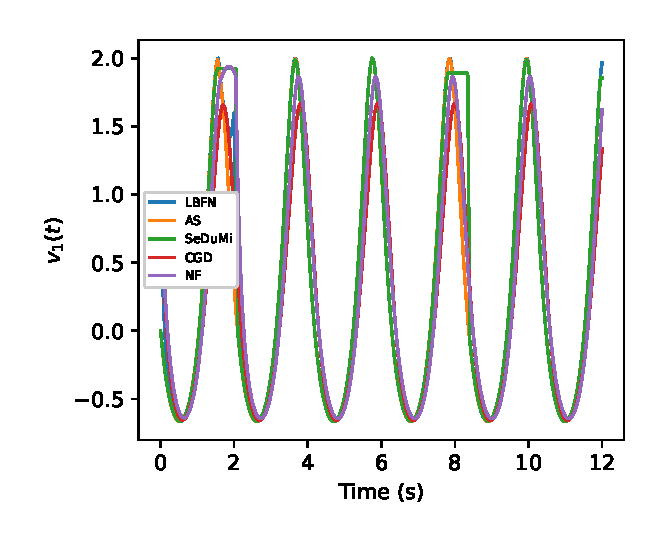
\includegraphics[width=58mm,height=46mm]{comp_x1.eps}}
\subfigure[]{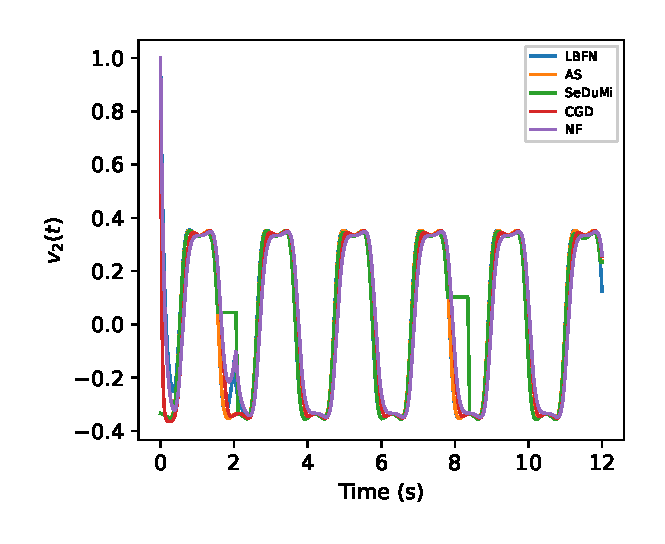
\includegraphics[width=58mm,height=46mm]{comp_x2.eps}}
\subfigure[]{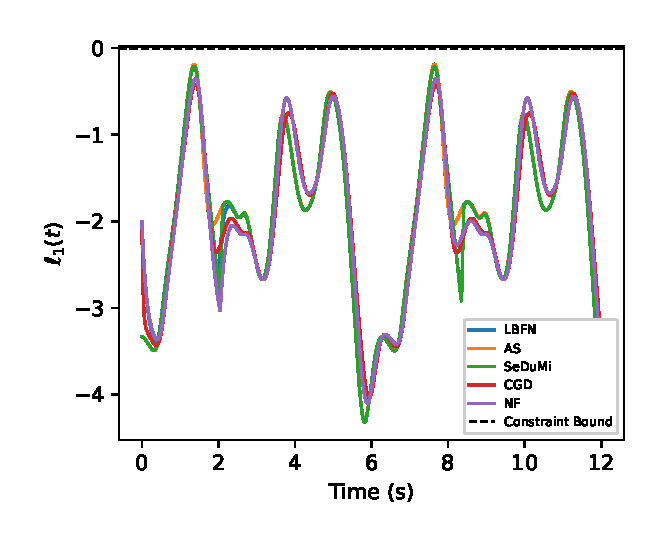
\includegraphics[width=58mm,height=46mm]{comp_g1.eps}}
\subfigure[]{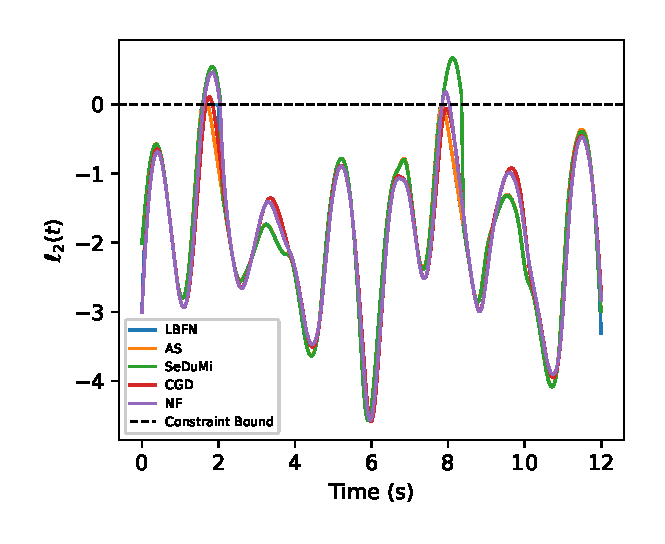
\includegraphics[width=58mm,height=46mm]{comp_g2.eps}}
\subfigure[]{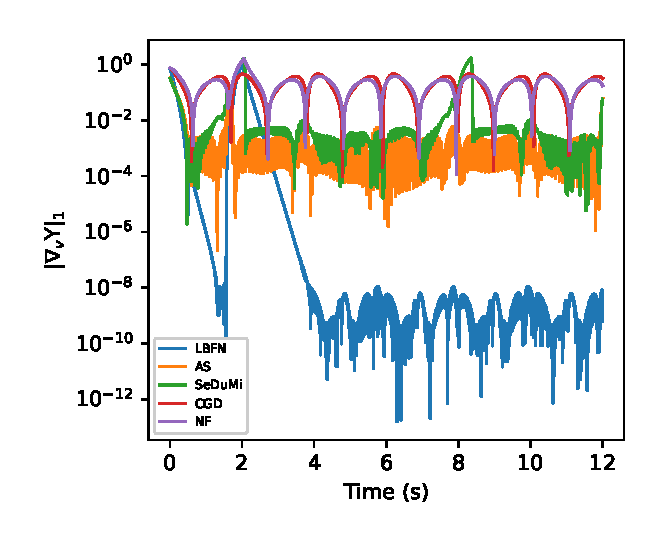
\includegraphics[width=58mm,height=46mm]{comp_err1.eps}}
\subfigure[]{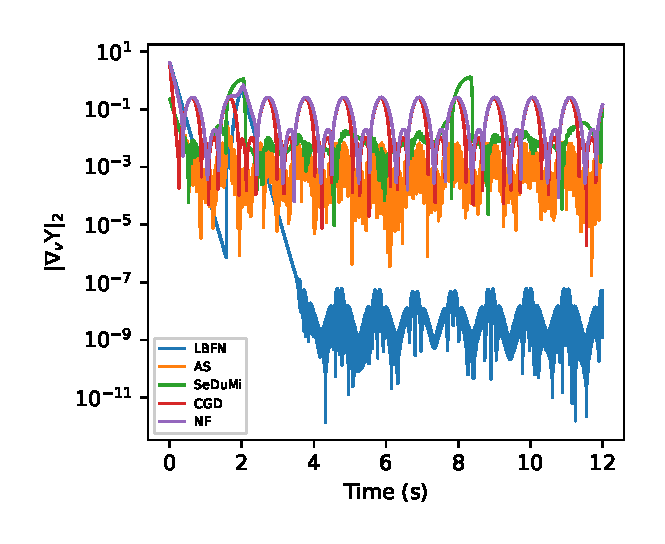
\includegraphics[width=58mm,height=46mm]{comp_err2.eps}}
\caption{Comparative simulation among the presented LBFN model \eqref{eq:full_dynamics}, the active-set (AS) approach, the SeDuMi approach \cite{SEDUME}, the continuous gradient descent (CGD) approach \cite{CGDSD}, and the Newton flows (NF) approach \cite{new1} for solving the DQP-IC problem \eqref{eq:problem234}, with $\alpha=10$, $\gamma_w=10$ and $\gamma_r=5$. (a) Convergence of $v_1(t)$. (b) Convergence of $v_2(t)$. (c) Constraint behavior of $g_1(t)$. (d) Constraint behavior of $g_2(t)$. (e) First entry of the absolute gradient error. (f) Second entry of the absolute gradient error.}
\label{Fg555}
\end{figure*}

\section{Experimental Results}\label{sec4}
This section provides two computational examples to demonstrate the effectiveness and advantages of the LBFN model.

\subsection{Numerical Example}\label{subsec41}
The quadratic objective function is designed to be strictly convex and dynamic through its parameters:
\begin{equation}\label{eq:objective}
\begin{aligned}
\hbar(\bm{v}(t) , t) = \frac{1}{2}
\begin{bmatrix} v_1(t) & v_2(t) \end{bmatrix}
\underbrace{\begin{bmatrix}
1 + 0.5 \sin (3t) & 0 \\
0 & 2 + \cos(6t)
\end{bmatrix}}_{\mathcal{P}(t)}
\begin{bmatrix} v_1(t)  \\ v_2(t)  \end{bmatrix} +\underbrace{\begin{bmatrix} \sin(3t) & \cos(3t) \end{bmatrix}}_{\bm{n}^T(t)}
\begin{bmatrix} v_1(t)  \\ v_2(t)  \end{bmatrix}
\end{aligned}
\end{equation}
which instantiates the generic problem \eqref{eq:problem} with $\mathcal{M}(t)\equiv\mathcal{P}(t)$ and $\bm{g}(t)\equiv\bm{n}(t)$. Notice that the Hessian matrix $\mathcal{P}(t)$ has a diagonal structure ensuring convexity. To be specific, $\mathcal{P}_{11}(t) = 1 + 0.5 \sin (3t)$ indicates periodic variation between $[0.5, 1.5]$, and $\mathcal{P}_{22}(t) = 2 + \cos(6t)$ indicates higher-frequency variation between $[1, 3]$. The eigenvalues of $\mathcal{P}(t)$ are $\lambda_1(t) \in [0.5, 1.5]$ and $\lambda_2(t) \in [1, 3]$. The problem remains strictly convex $\forall t \in \mathbb{R}$ because $\mathcal{P}(t) \succ 0$ and $\det(\mathcal{P}(t)) = (1 + 0.5 \sin (3t))(2 + \cos(6t))\geq 0.5 > 0$, which also guarantees a unique global minimum at each time instant.

Furthermore, the dynamic inequality constraints $\mathcal{G}(t)\bm{v}(t) \leq \bm{h}(t)$ are defined by:
\begin{equation}\label{eq:constraints}
\begin{aligned}
\begin{bmatrix}
\sin(2t) & 1 \\
-\cos(2t) & 2t/10 \\
\end{bmatrix}
\begin{bmatrix} v_1(t)  \\ v_2(t)  \end{bmatrix} \leq
\begin{bmatrix}
2 + \cos(2t) \\
2 - \sin(4t)
\end{bmatrix}
\end{aligned}
\end{equation}
so that this specific example is
\begin{equation}
\begin{aligned}
& \underset{\bm{v}(t) \in \mathbb{R}^n}{\text{minimize}} & & \hbar(\bm{v}(t), t) = \frac{1}{2} \bm{v}^\top(t) \mathcal{P}(t) \bm{v}(t) + \bm{n}^\top(t)\bm{v}(t) \\
& \text{subject to} & & \bm{\ell}(\bm{v}(t), t):\mathcal{G}(t)\bm{v}(t) \leq \bm{h}(t)
\end{aligned}
\label{eq:problem234}
\end{equation}

Convergence characteristics are comprehensively evaluated under varying convergence parameter $\alpha$, as shown in Figure~\ref{F333}, which reveals critical dynamics governing the system behavior. At $\alpha=2$, both variables $v_1(t)$ and $v_2(t)$ exhibit persistent oscillations that have not settled even by $t=3$~s, where the gradient-error norm remains of order $1$ ($9.2\times10^{-1}$), only decaying to $1.7\times10^{-2}$ by $t=5$~s. Increasing $\alpha$ sharply accelerates settling: at $t=0.2$~s the gradient-error norm is $8.4\times10^{-2}$ for $\alpha=20$ but only $5.1\times10^{-5}$ for $\alpha=5000$, and by $t=1$~s every case with $\alpha\geq20$ has already fallen below $2.3\times10^{-7}$, confirming the theoretically predicted exponential convergence rate proportional to $\alpha$. By $t=5$~s, all cases with $\alpha\geq20$ converge to a common floor between $3\times10^{-10}$ and $2\times10^{-9}$, indicating that the long-run floor visible in Figures~\ref{F333}(e)--(f) is governed by the fixed numerical precision of the barrier evaluation rather than by $\alpha$ itself once $\alpha$ is large enough for convergence to complete well within the simulated window. All five trajectories additionally show a brief, shared transient rise in gradient error around $t\approx1.6$--$2.0$~s, coinciding with a moment when the time-varying constraint boundary sweeps close to the tracked trajectory (visible as small excursions of $\ell_1(t)$ and $\ell_2(t)$ toward zero in Figures~\ref{F333}(c)--(d) at the same time), before the exponential decay resumes. In practice, $\alpha$ trades off settling speed against numerical stiffness: an excessively large $\alpha$ tightens the ODE's time constant and may require a correspondingly smaller integration step for a fixed-step numerical solver, a consideration we revisit in Section~\ref{sec5}.

Initialization robustness is rigorously tested across ten starting points, as shown in Figure~\ref{Fg3233}: nine sampled at random with $v_i(0)\in[-1.5,1.5]$, plus one deliberately infeasible starting point $\bm{v}(0)=(-3,4)$ for which $\bm{g}(0)=(1,1)>\bm{0}$ violates both constraints at $t=0$ by a margin of $1.0$ -- a direct computational test of the infeasible-initialization guarantee (Lemma~\ref{lem:wellposed}/Corollary~\ref{cor:tracking}) rather than only feasible starts. The LBFN model restores feasibility for this infeasible case within $0.05$~s ($\bm{g}(0.05)=(-1.76,-0.37)$), and the worst-case gradient-error norm across all ten starting points falls to $4.5\times10^{-2}$ by $t=0.3$~s and to $4.7\times10^{-7}$ by $t=1$~s. As in Figure~\ref{F333}, a brief transient rise occurs around $t\approx2$~s as the moving constraint boundary sweeps past several trajectories simultaneously (worst-case gradient-error norm $1.3$, worst-case constraint value $2\times10^{-4}$, i.e., an essentially negligible boundary touch), after which convergence resumes and the worst-case gradient-error norm falls to $3.1\times10^{-9}$ by $t=3$~s -- a reduction of $8.9$ to $9.7$ orders of magnitude from each trajectory's initial value -- establishing the approach's robustness against both initialization variance and initial infeasibility, a desirable property for computing systems where the optimizer may be restarted or hot-swapped at an arbitrary, possibly infeasible, state.

Comparative analysis against established solvers revealed the LBFN model's superior performance in dynamic programming problems, as shown in Figure~\ref{Fg555}. The comparative approaches include the active-set (AS) approach \cite{act-se}, the continuous gradient descent (CGD) approach \cite{CGDSD}, the SQP approach \cite{SQP34}, the SeDuMi interior-point approach \cite{SEDUME}, and the Newton flows (NF) approach \cite{new1}. Specifically, the SeDuMi and NF approaches show the largest constraint violations, peaking at $6.7\times10^{-1}$ and $4.7\times10^{-1}$ respectively, during two transition windows ($t\in[1.6,2.1]$~s and $t\in[7.8,8.4]$~s); the AS and CGD approaches show smaller, single-window violations (peaking at $3.7\times10^{-3}$ and $1.1\times10^{-1}$ respectively, near $t\approx1.6$--$1.8$~s), and the CGD approach additionally develops a persistent steady-state offset rather than decaying (median gradient-error norm $2.5\times10^{-1}$ over $t\in[2,12]$~s); the LBFN model's own trajectory only briefly touches the constraint boundary during the same transition windows, with a peak excursion of $5.3\times10^{-3}$ -- two orders of magnitude smaller than SeDuMi/NF and consistent with the numerical precision of the barrier evaluation (Section~\ref{subsec31}) rather than a genuine, sustained loss of feasibility. Gradient-error convergence metrics confirm distinct advantages: by $t=12$~s the LBFN model's gradient-error norm has decayed to $1.4\times10^{-9}$ (median $6.7\times10^{-9}$ over $t\in[2,12]$~s), while the AS, SeDuMi, CGD, and NF baselines remain at $1.3\times10^{-1}$, $1.3\times10^{-1}$, $3.5\times10^{-1}$, and $2.2\times10^{-1}$ respectively at the same instant -- four to five orders of magnitude higher. These results confirm the theoretical predictions of global convergence with tunable rates and persistent feasibility.

\subsection{Application to Dynamic Robot Navigation}\label{subsec42}
In this part, to further verify the effectiveness of the constructed LBFN model as a real-time computing primitive, a dynamic robot navigation task is designed, in which the robot is required to track a dynamic target in real time. The task is formulated as an inequality-constrained dynamic program with a non-quadratic (Gaussian repulsive potential) objective, to which the general LBFN dynamics of Section~\ref{sec2} apply directly:
\begin{equation}\label{eq:robot}
\begin{aligned}
& \underset{\bm{p}(t) \in \mathbb{R}^2}{\text{minimize}}~~~ \frac{1}{2}k_t\|\bm{p}(t)-\bm{p}_{Tar}(t)\|^2+\sum_{i=1}^7\exp\left(-\frac{\|\bm{p}(t)-\bm{p}_{Obs_i}(t)\|^2}{k_i}\right),\\
&\text{subject to} ~~~\mathcal{A}\bm{p}(t)\leq\bm{d}
\end{aligned}
\end{equation}
where $\bm{p}(t)\in\mathbb{R}^2$ denotes the robot's planar position (a specific instance of the decision variable $\bm{v}(t)$ in \eqref{eq:problem} for $n=2$), $\mathcal{A}=[1~0;0~1;-1~0;0~-1]$ and $\bm{d}=[100;100;0;0]$, so that this inequality denotes the physical bounds of the navigation map. The LBFN model's convergence parameter $\alpha$ is set to $1000$, guaranteeing swift convergence and meeting the real-time control requirement of the task \eqref{eq:robot}. The moving target's trajectory is $\bm{p}_{Tar}(t)=[50+40\sin(0.25t),\,50+25\cos(0.25t)]^{\top}$. The 7 obstacles $\bm{p}_{Obs_i}(t)$, $i=1,\dots,7$, are located at $[20;25]$~m, $[60;20]$~m, $[70;60]$~m, $[50;85]$~m, $[30;72]$~m, $[38;35]$~m and $[90;40]$~m, with parameters $k_1=0.8$, $k_2=0.6$, $k_3=1.0$, $k_4=1.2$, $k_5=1.2$, $k_6=0.8$, $k_7=0.9$, and $k_t=0.3$. The task duration is $T=30$~s.

As depicted in Figure~\ref{F333vv3}, snapshots at $t=10$~s, $t=20$~s, and $t=30$~s illustrate the experimental results. The dynamic target moves along an elliptical trajectory, with seven stationary obstacles in the map. Figures~\ref{F333vv3}(a), (d), and (g) show the trajectory-tracking result, where the robot starts from its initial point (initially $76.3$~m from the moving target) and swiftly converges to the moving target, closing to within $0.01$~m by $t=1$~s and effectively $0$~m by $t=5$~s, and then follows the target in real time while avoiding obstacles (the closest robot-obstacle approach over the entire $30$~s run is $1.53$~m, near obstacle 5 at $t\approx23$~s, and the robot remains within the map's $[0,100]\times[0,100]$ bounds throughout). Figures~\ref{F333vv3}(b), (e), and (h) show the potential force field on a contour plot, and Figures~\ref{F333vv3}(c), (f), and (i) show the potential-function landscape, for the three time instants. This demonstrates that, under the LBFN model, the robot's onboard computation excellently accomplishes the given dynamic navigation task in real time.

\begin{figure*}[thbp]\centering
\subfigure[]{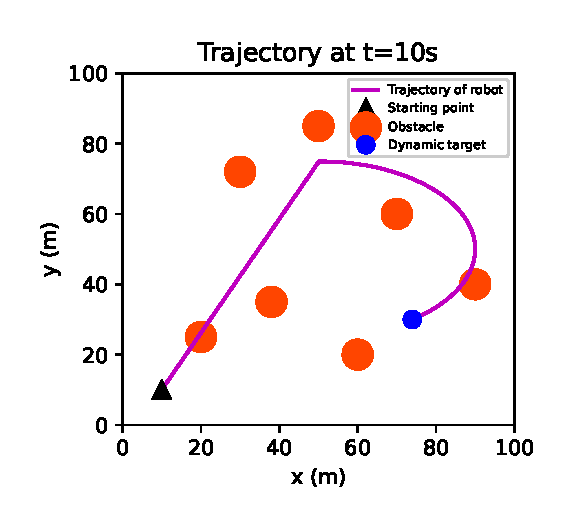
\includegraphics[width=40mm,height=34mm]{t10_motion.eps}}
\subfigure[]{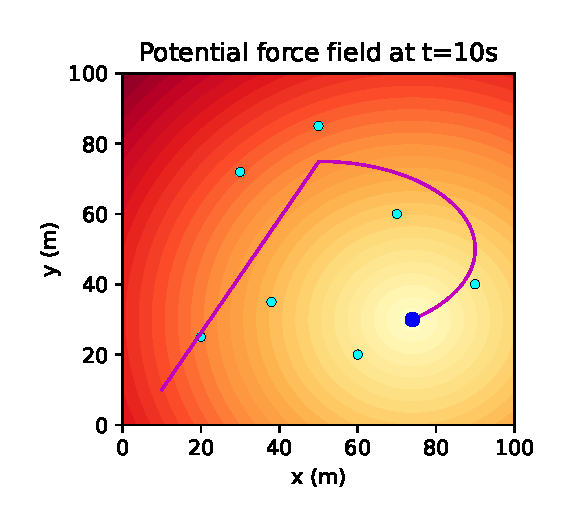
\includegraphics[width=40mm,height=34mm]{t10_contour.eps}}
\subfigure[]{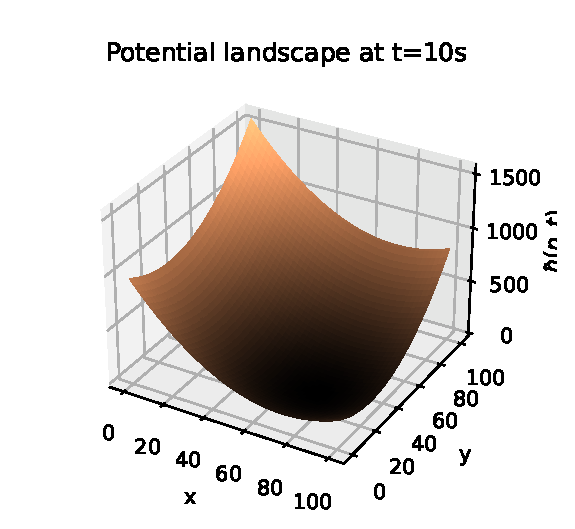
\includegraphics[width=40mm,height=34mm]{t10_land.eps}}
\subfigure[]{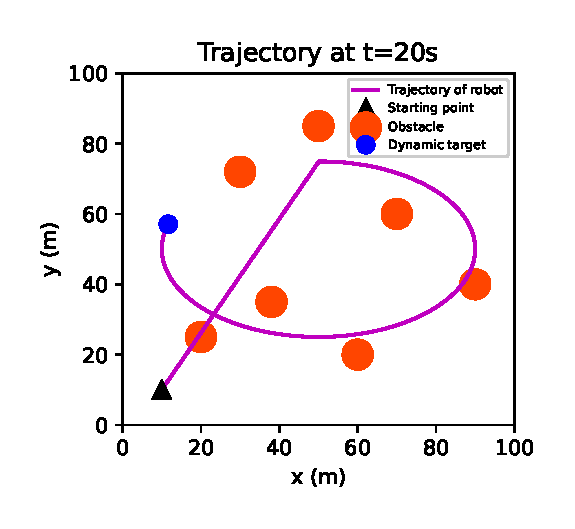
\includegraphics[width=40mm,height=34mm]{t20_motion.eps}}
\subfigure[]{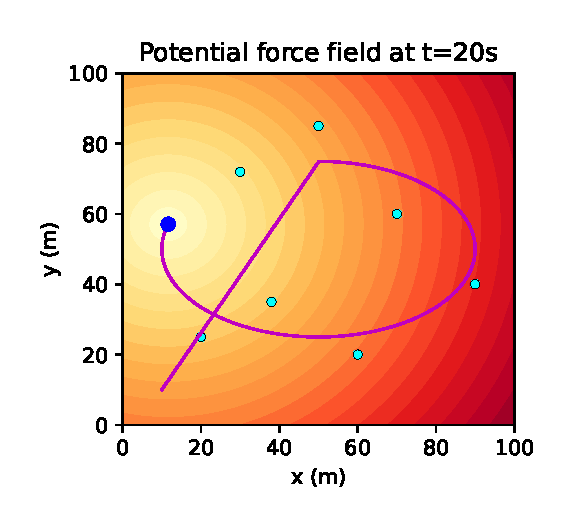
\includegraphics[width=40mm,height=34mm]{t20_contour.eps}}
\subfigure[]{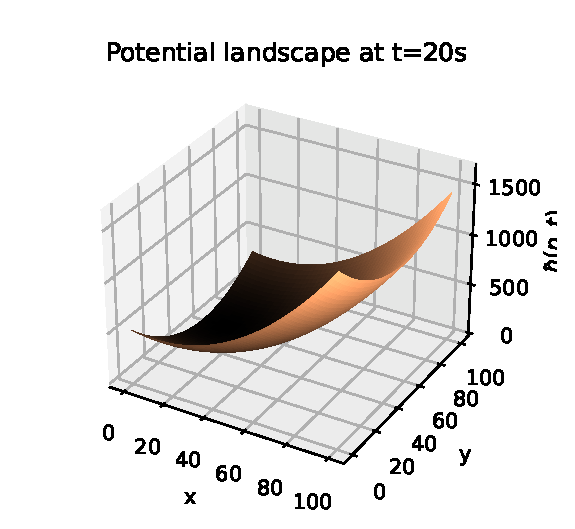
\includegraphics[width=40mm,height=34mm]{t20_land.eps}}
\subfigure[]{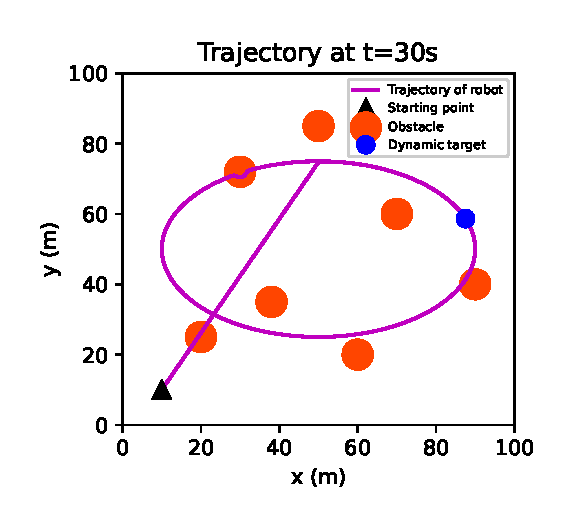
\includegraphics[width=40mm,height=34mm]{t30_motion.eps}}
\subfigure[]{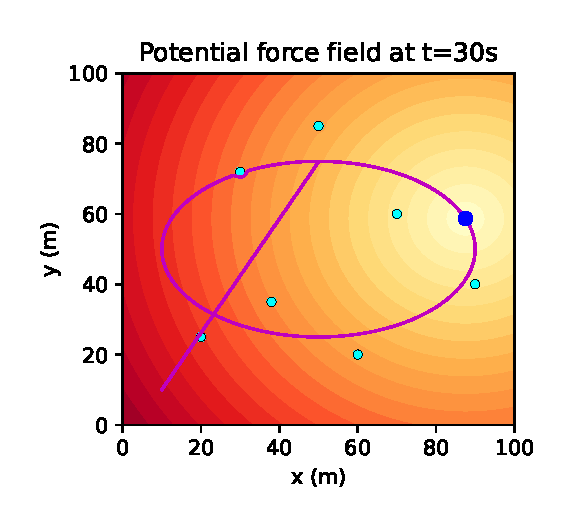
\includegraphics[width=40mm,height=34mm]{t30_contour.eps}}
\subfigure[]{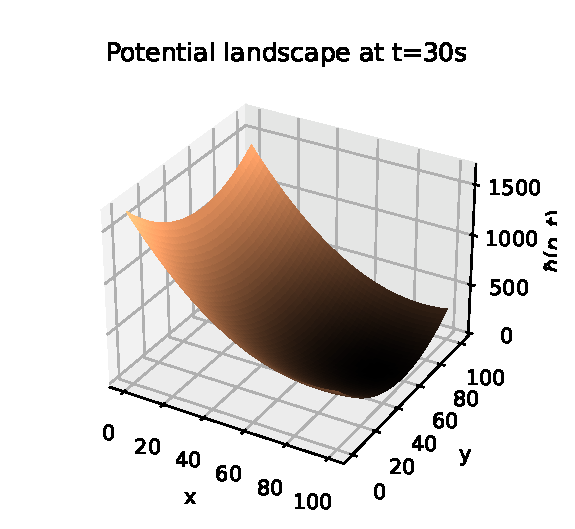
\includegraphics[width=40mm,height=34mm]{t30_land.eps}}
\caption{Experimental results of the dynamic robot navigation task \eqref{eq:robot} accomplished by the LBFN model in real time, task duration $T=30$~s, involving 7 obstacles. (a) Trajectory at $t=10$~s. (b) Potential force field at $t=10$~s. (c) Potential landscape at $t=10$~s. (d)--(f) Same at $t=20$~s. (g)--(i) Same at $t=30$~s.}
\label{F333vv3}
\end{figure*}

\section{Limitations and Future Work}\label{sec5}
While the LBFN model demonstrates strong theoretical guarantees and empirical performance, several limitations delineate directions for future research relevant to its deployment as a computing primitive. First, although Section~\ref{sec2} shows that Lemma~\ref{lem:wellposed}, Theorem~\ref{thm:main}, and Corollary~\ref{cor:tracking} extend verbatim from the quadratic case \eqref{eq:problem} to any objective that is $m_f$-strongly convex in $\bm{v}(t)$ for every $t$, this still excludes objectives that are only \emph{locally} convex, such as the Gaussian repulsive potential used in Section~\ref{subsec42}, whose Hessian can lose positive definiteness near an obstacle; extending the convergence guarantees to such locally nonconvex, or more generally nonconvex, dynamic programs would broaden applicability but requires new arguments beyond the strong-convexity-based Lyapunov analysis of Section~\ref{sec3}. Second, the model assumes that $\mathcal{M}(t)$, $\bm{g}(t)$, $\mathcal{N}(t)$, $\bm{d}(t)$ and their time derivatives are known in closed form; in practice these quantities are often estimated from noisy sensor data, so coupling the LBFN dynamics with derivative estimators or observer-based prediction would be necessary for deployment on physical hardware. Third, although Section~\ref{subsec31} shows the per-instant cost scales as $O(n^3+pn^2)$, this remains cubic in the state dimension $n$; for large-scale problems, exploiting the Sherman--Morrison--Woodbury identity for the rank-$p$ Hessian update, warm-started or incremental Cholesky factorizations across nearby time instants, or distributed/parallel implementations across constraint blocks are promising ways to reduce this cost further on multi-core or edge-computing hardware. Fourth, the barrier parameter $w(t)=w(0)e^{\gamma_w t}$ grows without bound, which is necessary for asymptotic exactness but can induce numerical ill-conditioning of $\nabla_{\bm{vv}}\Upsilon$ near the constraint boundary over long horizons; adaptive or saturating barrier schedules merit investigation for long-duration deployments. Finally, the robot navigation case study in Section~\ref{subsec42} is validated in simulation; hardware-in-the-loop and physical robot experiments, together with benchmarking on higher-dimensional and multi-agent DQP-IC instances, are natural next steps to further substantiate the real-time computing applicability of the proposed model.

\section{Conclusion}\label{sec6}
This paper has established a logarithmic barrier function-based Newton's (LBFN) computational model for real-time solving of dynamic quadratic programming problems subject to inequality constraints. The proposed model fundamentally advances beyond traditional approaches by employing parametric adaptive log-barrier functions to directly handle inequality constraints, thereby avoiding the auxiliary variables typically required by KKT-based methods. We established the well-posedness of the resulting continuous-time dynamics, proved global asymptotic stability with an exponentially decaying, tunable tracking error via a Lyapunov argument, and derived a per-instant computational complexity of $O(n^3+pn^2)$ comparable to a single Newton step on a static quadratic program of the same size. These properties make the model particularly suitable for real-time computing environments where both computational efficiency and constraint adherence are critical. Numerical experiments comprehensively validated the model's performance, showing superior convergence speed and solution accuracy compared to active-set, sequential quadratic programming, interior-point, continuous gradient-descent, and Newton-flow baselines, while a dynamic robot navigation case study demonstrated simultaneous trajectory tracking and obstacle avoidance in real-time operation. Building on the limitations discussed in Section~\ref{sec5}, future work will extend the LBFN framework to nonlinear and nonconvex dynamic programs, incorporate noise-robust parameter estimation, exploit factorization-update techniques for large-scale and distributed computing deployments, and pursue hardware validation on physical robotic and embedded computing platforms.

\backmatter

\bmhead{Acknowledgments}
Not applicable.

\section*{Declarations}

\begin{itemize}
\item \textbf{Funding:} This research received no external funding.
\item \textbf{Conflict of interest/Competing interests:} The authors declare no competing interests.
\item \textbf{Ethics approval:} Not applicable. This study did not involve human participants, human data, or animals.
\item \textbf{Consent to participate:} Not applicable.
\item \textbf{Consent for publication:} Not applicable.
\item \textbf{Availability of data and materials:} The data generated and analysed during the current study, together with the scripts that reproduce the numerical experiments and figures, are available in the GitHub repository at \url{https://github.com/yzhou364/LBFN}.
\item \textbf{Code availability:} The Python implementation of the LBFN model and all baseline solvers is available in the GitHub repository at \url{https://github.com/yzhou364/LBFN}.
\item \textbf{Authors' contributions:} Y.Z. conceived the research idea, supervised the study, and revised the manuscript; Y.Z. is the corresponding author. J.W. developed the theoretical framework, implemented the LBFN algorithm, conducted the numerical simulations and the robot navigation experiment, and drafted the manuscript. Both authors reviewed and approved the final version of the manuscript.
\item \textbf{Use of AI:} An AI assistant (Claude, Anthropic) was used to assist with implementing the numerical simulation code, carrying out the numerical experiments reported in Section~\ref{sec4}, and drafting and revising the manuscript text. The authors designed the study, verified the correctness of the implementation and results, and take full responsibility for the content of this manuscript.
\end{itemize}

\begin{thebibliography}{99}

\bibitem{ldfy} D. Liu, S. Xue, B. Zhao, B. Luo and Q. Wei, ``Adaptive Dynamic Programming for Control: A Survey and Recent Advances," \emph{IEEE Transactions on Systems, Man, and Cybernetics: Systems}, vol. 51, no. 1, pp. 142--160, Jan. 2021.

\bibitem{acces23} Y. E. Wang, ``Theory of Broadband Transmission of Frequency Modulated Signals through High-Q Resonators with Continuous Time-Varying Matching Networks," \emph{IEEE Access}, doi: 10.1109/ACCESS.2025.3595056.

\bibitem{trp2024} D. Hanover, A. Loquercio, L. Bauersfeld, A. Romero, R. Penicka, Y. Song, G. Cioffi, E.  Kaufmann and D. Scaramuzza, ``Autonomous Drone Racing: A Survey," \emph{IEEE Transactions on Robotics}, vol. 40, pp. 3044--3067, May 2024.

\bibitem{acceess4} J. Park, M. Kang, Y. Lee, J. Jung, H. -T. Choi and J. Choi, ``Multiple Autonomous Surface Vehicles for Autonomous Cooperative Navigation Tasks in a Marine Environment: Development and Preliminary Field Tests," \emph{IEEE Access}, vol. 11, pp. 36203--36217, 2023.

\bibitem{trp2025} K. Harlow, H. Jang, T. D. Barfoot, A. Kim and C. Heckman, ``A New Wave in Robotics: Survey on Recent MmWave Radar Applications in Robotics," \emph{IEEE Transactions on Robotics}, vol. 40, pp. 4544--4560, Sept. 2024.

\bibitem{titis333} Y. Liufu et al., ``Collaborative Physics-Informed Neural Dynamics Approach for Autonomous Vehicles with Nonconvex Safety-Critical Constraints", \emph{IEEE Transactions on Intelligent Transportation Systems}, doi: 10.1109/TITS.2025.3572336.

\bibitem{acces345} J. Nur Fadila, N. Haliza Abdul Wahab, A. Alshammari, A. Aqarni, A. Al-Dhaqm and N. Aziz, ``Comprehensive Review of Smart Urban Traffic Management in the Context of the Fourth Industrial Revolution,"  \emph{IEEE Access}, vol. 12, pp. 196866--196886, 2024.

\bibitem{titis2} C. Cre$\beta$, Z. Bing and A. C. Knoll, ``Intelligent Transportation Systems Using Roadside Infrastructure: A Literature Survey," \emph{IEEE Transactions on Intelligent Transportation Systems}, vol. 25, no. 7, pp. 6309--6327, Jul. 2024.

\bibitem{tesagf} M. N. Elsayed, O. De Silva, A. Jayasiri, G. K. I. Mann and R. Gosine, ``Optimization-Based Maneuvering Target Tracking Using Multiple Model Horizon Scenario Tree With Model Interaction," \emph{IEEE Transactions on Aerospace and Electronic Systems}, doi: 10.1109/TAES.2025.3592177.

\bibitem{acceess3} G. R. Prudhvi Kumar and S. Dasarathan, ``Metaheuristic-Tuned Droop Control for PV-Based DC Microgrid Optimization Under Dynamic Load Conditions," \emph{IEEE Access}, doi: 10.1109/ACCESS.2025.3592751.

\bibitem{TSTT12} J. Fan, L. Jin, P. Li, J. Liu, Z.-G. Wu and W. Chen, ``Coevolutionary Neural Dynamics Considering Multiple Strategies for Nonconvex Optimization," \emph{Tsinghua Science and Technology}, doi: 10.26599/TST.2025.9010120.

\bibitem{tiify}  Y. Liufu et al., ``Modified Gradient Projection Neural Network for Multiset Constrained Optimization,"  \emph{IEEE Transactions on Industrial Informatics}, vol. 19, no. 9, pp. 9413--9423, Sept. 2023.

\bibitem{siam1} J. M. Altschuler, J. Bok and K. Talwar, ``On the Privacy of Noisy Stochastic Gradient Descent for Convex Optimization," \emph{SIAM Journal on Computing}, vol. 53, no. 4, 969--1001, 2024.

\bibitem{hwx2} H. Wen and X. He, ``Arbitrary-Time Stable Gradient Flows Using Neurodynamic System for Continuous-Time Optimization," \emph{IEEE Transactions on Circuits and Systems II: Express Briefs}, vol. 70, no. 12, pp. 4559--4563, Dec. 2023.

\bibitem{aces355} R. Chen and X. Li, ``Implicit Runge-Kutta Methods for Accelerated Unconstrained Convex Optimization," \emph{IEEE Access}, vol. 8, pp. 28624--28634, 2020.

\bibitem{trone3} Jing Ren, K. A. McIsaac and R. V. Patel, ``Modified Newton's Method Applied to Potential Field-Based Navigation for Mobile Robots," \emph{IEEE Transactions on Robotics}, vol. 22, no. 2, pp. 384--391, Apr. 2006.

\bibitem{newt1} D. Niu, Y. Hong and E. Song, ``A Dual Inexact Nonsmooth Newton Method for Distributed Optimization," \emph{IEEE Transactions on Signal Processing}, vol. 73, pp. 188--203, 2025.

\bibitem{act-se33} H. Kim and H. Park, ``Nonnegative Matrix Factorization Based on Alternating Nonnegativity Constrained Least Squares and Active Set Method," \emph{SIAM Journal on Matrix Analysis And Applications}, vol. 30, no. 2, pp. 713--730. 2008.

\bibitem{act-se} G. Cimini and A. Bemporad, ``Exact Complexity Certification of Active-Set Methods for Quadratic Programming," \emph{IEEE Transactions on Automatic Control}, vol. 62, no. 12, pp. 6094--6109, Dec. 2017.

\bibitem{SQP34} F. E. Curtis and M. L. Overton, ``A Sequential Quadratic Programming Algorithm for Nonconvex, Nonsmooth Constrained Optimization," \emph{SIAM Journal on Optimization}, vol. 22, no. 2, pp. 474--500. 2012.

\bibitem{SQP3444} A. S. Berahas, M. Xie and B. Zhou, ``A Sequential Quadratic Programming Method With High-Probability Complexity Bounds for Nonlinear Equality-Constrained Stochastic Optimization," \emph{SIAM Journal on Optimization}, no. 35, no. 1, pp. 240--269, 2025.

\bibitem{S22} X. Shi, X. Xu, J. Cao, and X. Yu, ``Finite-Time Convergent Primal-Dual Gradient Dynamics With Applications to Distributed Optimization," \emph{IEEE Transactions on Cybernetics}, vol. 53, no. 5, pp. 3240--3252, May 2023.

\bibitem{S44} J. I. Poveda and M. Krstic, ``Fixed-time Gradient-Based Extremum Seeking," in Proceedings of the American Control Conference, 2020, pp. 2838--2843.

\bibitem{S4456} I. Fatkhullin and B. Polyak, ``Optimizing Static Linear Feedback: Gradient Method," \emph{SIAM Journal on Control and Optimization}, vol. 59, no. 5, pp. 3887--3911, 2021.

\bibitem{nn34} M. Mestari, M. Benzirar, N. Saber and M. Khouil, ``Solving Nonlinear Equality Constrained Multiobjective Optimization Problems Using Neural Networks," \emph{IEEE Transactions on Neural Networks and Learning Systems}, vol. 26, no. 10, pp. 2500--2520, Oct. 2015.

\bibitem{S4fw4} T. Breiten and L. Pfeiffer, ``On the Turnpike Property and The Receding-Horizon Method for Linear-Quadratic Optimal Control Problems," \emph{SIAM Journal on Control and Optimization}, vol. 58, no. 2, pp. 1077--1102, 2020.

\bibitem{rbmm} Y. Hu, L. Wei, X. Guo, Z. Li, Y. Wei, and Q. Fang, ``Priority-Based Reward Mechanism for Dual-Robot Path Planning in Dynamic Environments," \emph{IEEE Access}, vol. 13, pp. 92519-92530, 2025.

\bibitem{rbm3Rm}  M. Liu, Y. Li, Y. Chen, Y. Qi, and L. Jin, ``A Distributed Competitive and Collaborative Coordination for Multirobot Systems," \emph{IEEE Transactions on Mobile Computing}, vol. 23, no. 12, pp. 11436-11448, Dec. 2024.

\bibitem{rbmmr4} R. J. Roesthuis and S. Misra, ``Steering of Multisegment Continuum Manipulators Using Rigid-Link Modeling and FBG-Based Shape Sensing," \emph{IEEE Transactions on Robotics}, vol. 32, no. 2, pp. 372--382, Apr. 2016.

\bibitem{xy111} J. Lin, D.-H. Zhai, Y. Xiong and Y. Xia, ``Safety Control for UR-Type Robotic Manipulators via High-Order Control Barrier Functions and Analytical Inverse Kinematics,"  \emph{IEEE Transactions on Industrial Electronics}, vol. 71, no. 6, pp. 6150--6160, Jun. 2024.

\bibitem{tiv124} S. Jing, Y. Zhao, X. Zhao, F. Hui and A. J. Khattak, ``An Efficient High-Risk Lane-Changing Scenario Edge Cases Generation Method for Autonomous Vehicle Safety Testing," \emph{IEEE Transactions on Intelligent Vehicles}, vol. 10, no. 1, pp. 459--471, Jan. 2025.

\bibitem{lj11} L. Jin, L. Wei, and S. Li, ``Gradient-Based Differential Neural-Solution to Time-Dependent Nonlinear Optimization," \emph{IEEE Transactions on Automatic Control}, vol. 68, no. 1, pp. 620--627, Jan. 2023.

\bibitem{lfyy12} Y. Liufu et al., ``Adaptive Noise-Learning Differential Neural Solution for Time-Dependent Equality-Constrained Quadratic Optimization," \emph{IEEE Transactions on Neural Networks and Learning Systems}, doi: 10.1109/TNNLS.2025.3561415.

\bibitem{book12} S. Boyd and L. Vandenberghe, Convex Optimization. Cambridge, U.K.: Cambridge Univ. Press, 2004.

\bibitem{CGDSD} J. Sirignano and K. Spiliopoulos, ``Stochastic Gradient Descent in Continuous Time," \emph{SIAM Journal on Financial Mathematics}, vol. 8, no. 1, pp. 933--961, 2017.

\bibitem{SEDUME} Y. Labit, D. Peaucelle and D. Henrion, ``SeDuMi Interface 1.02: A tool for Solving LMI Problems with SeDuMi," in Proceedings. IEEE International Symposium on Computer Aided Control System Design. IEEE, 2002: 272--277.

\bibitem{new1} D. Niu, Y. Hong and E. Song, ``A Dual Inexact Nonsmooth Newton Method for Distributed Optimization," \emph{IEEE Transactions on Signal Processing}, vol. 73, pp. 188--203, 2025.

\end{thebibliography}

\end{document}
